\section{Design}
\label{sec:Design}

\subsection{Architecture Design}
Because we selected the web application model from the beginning, so the classic client-server architecture was quickly adopted, which is a distributed application structure that partitions tasks or workloads between the providers of a resource or service, called servers, and service requesters, called clients. In theory, any device connected to the Internet can try to access and obtain the resources or services of the server while the server is running normally. Figure \ref{Client-Server Architecture} shows how it works.

\begin{figure}[htb]
\centering
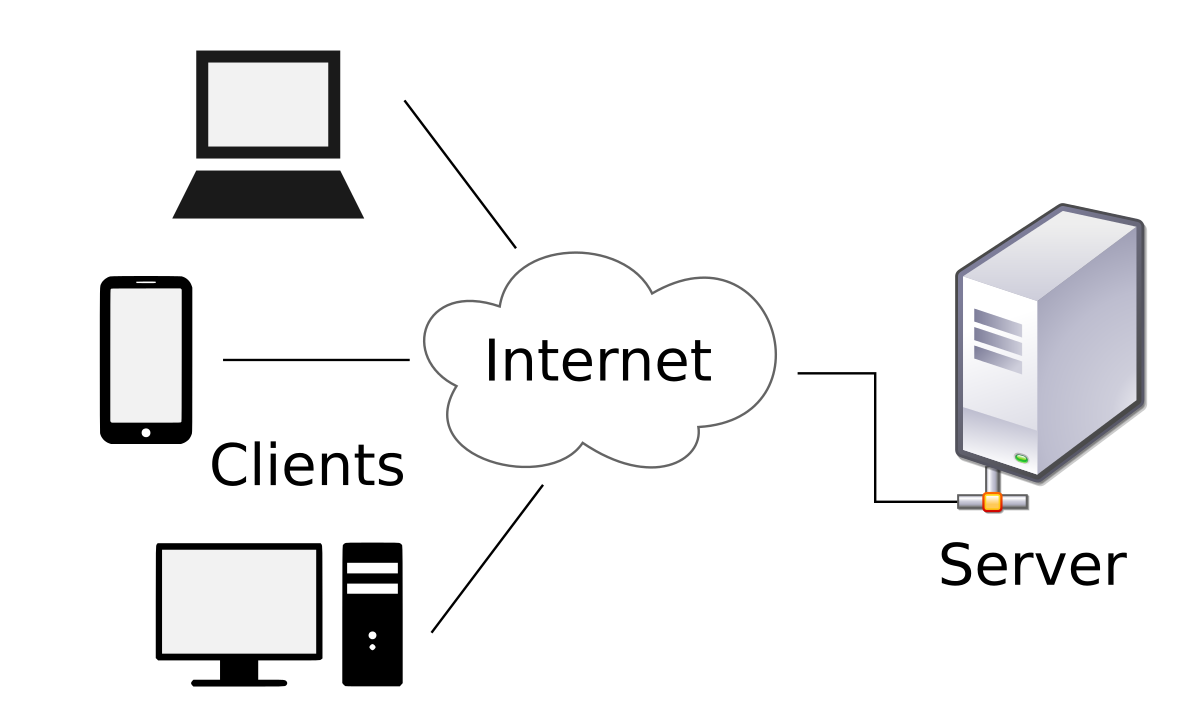
\includegraphics[width=\textwidth]{section03/assets/client_server.png}
\caption[the Architecture of Client-Server Model]{\label{Client-Server Architecture}the Architecture of Client-Server Model}
\end{figure}

Based on the client-server structure, we have detailed its component structures below:
\subsubsection{Web Browser or Client}
The web browser or client is the interface rendition of a web app functionality, with which the user interacts with. This content delivered to the client can be developed using HTML, JavaScript, and CSS and doesn’t require operating system related adaptations. In essence, the web browser or client manages how end users interact with the application.

There are three, well-known Web Application Architecture types available in the modern tech landscape: Single Page Applications (SPA), Microservices, and Serverless Architectures. Considered the needs of the project and the choice of the software development life cycle model, we chose the SPA architecture.

The SPA model interacts with the user in a more dynamic fashion by providing updated content within the current page, rather than loading entirely new pages from the server with each action from the user. It helps prevent interruptions in the user experience, transforming the behavior of the application such that it resembles a traditional desktop application.

\subsubsection{Web Application Server}
The web application server manages business logic and data persistence and can be built using PHP, Python, Java, Ruby, .NET, Node.js, among other languages. It’s comprised of at least a centralized hub or control center to support multi-layer applications. The essential purpose of a web server architecture is to complete requests made by clients for a website. The clients are typically browsers and mobile apps that make requests using secure HTTPs protocol, either for page resources or a REST API.

Since the focus of this project is on the client side (frontend), which is the map generator (written in JavaScript), so we chose the Node.js Express framework. Moreover the Node.js is written using JavaScript and is the same technology as frontend components, which makes it easier for the developer to program backend services and frontend user interfaces. It also provides consistency, code sharing and reusability, simple knowledge-transfer, and a large number of free tools. These benefits bring flexibility and efficiency when building this project.

\subsubsection{Database Server}
The database server provides and stores relevant data for the application. Additionally, it may also supply the business logic and other information that is managed by the web application server. There are multiple popular databases systems available: Oracle, MySQL, Microsoft SQL Server, PostgreSQL, MongoDB, MariaDB, DB2, and SAP HANA.

Since the project involves a small number of entities and the relationships among entities are not complicated, so we chose the MongoDB, which is dynamic, flexible and easy to get started, it also provides high performance, high availability, and high scalability. What's more, our main purpose is to save maps and implement basic CRUD (create, retrieve, update, delete) operations of the database. As MongoDB is a schema-less database (written in C++), we can serialize the map data to JSON, send it to MongoDB and then save it.

\subsection{Database Design}

\subsection{REST API Design}
\begin{table}[ht]
  \centering
  \begin{tabularx}{\textwidth}{>{\raggedright}cXX} % way of defining a fix columns width
    \toprule[1.5pt]
    \textbf{HTTP Verb} & \textbf{URI} & \textbf{Description}
    \\ \midrule[1.5pt]
    POST & /metro/auth/signup & Sign up for a new account
    \\ \midrule
    POST & /metro/auth/login & Log in to the system
    \\ \midrule
    POST & /metro/auth/logout & Log out of the system
    \\ \midrule
    GET & /metro/api/v1/users & Get a list of all users
    \\ \midrule
    GET & /metro/api/v1/users/\{id\} & Get the user with \{id\}
    \\ \midrule
    GET & /metro/api/v1/users/\{uid\}/ maps & Get a list of all maps of the user with \{uid\}
    \\ \midrule
    PATCH & /metro/api/v1/users/\{id\}/ password & Verify the password of the user with \{id\}
    \\ \midrule
    PUT & /metro/api/v1/users/\{id\}/ password & Update the password of the user with \{id\}
    \\ \midrule
    PUT & /metro/api/v1/users/\{id\}/ email & Update the email of the user with \{id\} \\ \midrule
    PUT & /metro/api/v1/users/\{id\}/ name & Update the name of the user with \{id\} \\ \midrule
    PUT & /metro/api/v1/users/\{id\}/ enabled & Update the enabled of the user with \{id\}
    \\ \midrule
    GET & /metro/api/v1/maps/\{id\} & Get the map with \{id\}
    \\ \midrule
    GET & /metro/api/v1/maps/ ?page=\{page\}\&limit=\{limit\} & Get a list of \{limit\} maps on page \{page\}
    \\ \midrule
    POST & /metro/api/v1/maps & Add a new map to the database
    \\ \midrule
    PUT & /metro/api/v1/maps/\{id\} & Update the map with \{id\}
    \\ \midrule
    DELETE & /metro/api/v1/maps/\{id\} & Delete the map with \{id\}
    \\ \bottomrule[1.5pt]
  \end{tabularx}
  \caption[REST API Design Table]{REST API Design Table}
  \label{REST API Design Table}
\end{table}

\subsection{Map Generator Design}
